\documentclass[12pt,aspectratio=169]{beamer}
\usepackage[utf8]{inputenc}
\usepackage[T1]{fontenc}
\usepackage{lmodern}
\usepackage{url}

\usepackage{multirow}

\usepackage{caption}

% Beamer theme
\usetheme{metropolis}

% Change English font
\setsansfont{TeX Gyre Adventor}

% Japanese font
\usepackage{xeCJK}
\setCJKmainfont{ipaexm.ttf} % IPAexMincho
\setCJKsansfont{ipaexg.ttf} % IPAexGothic

% Furigana
\usepackage{pxrubrica}

% Spacing
\usepackage{setspace}
\setstretch{1.6}

% Environment Settings
\newenvironment{items}
	{\begin{itemize}
		\setlength\itemsep{5pt}
	}{\end{itemize}}


\begin{document}
	\author{Takeshi (\ruby[g]{綾小路}{あやのこうじ}\ruby{武}{たけし})}
	\title{Kanji Lesson by Takeshi}
	\subtitle{Class 1: Introduction}
	%\logo{}
	\institute{TV Takeshi}
	\date{}
	%\subject{}
	%\setbeamercovered{transparent}
	%\setbeamertemplate{navigation symbols}{}
	\begin{frame}[plain]
		\maketitle
	\end{frame}

	\section{Table of contents}
	
	\begin{frame}{Contents}
		\begin{items}
			\item About the instructor
			\item Introduction to the class
			\item Kanji basics: Part 1
			\begin{items}
				\item What is Kanji?
				\item Classifications of Kanji
			\end{items}
		\end{items}
	\end{frame}

	\section{Introduction}

	\begin{frame}{About the instructor}
		\begin{items}
			\item Alias: Takeshi Ayanokoji (\ruby[g]{綾小路}{あやのこうじ}\ruby{武}{たけし})
			\item You can call me \textbf{Takeshi}.
			\item Final degree: Bachelor of Economics (Osaka University)
			\item Certifications
			\begin{items}
				\item JLPT N1
				\item Kanji Kentei Level 2 (\ruby{漢字検定}{かん|じ|けん|てい}; Kanji Aptitude Test)
			\end{items}
		\end{items}
	\end{frame}

	\begin{frame}{Introduction}
		\begin{items}
			\item Objective: "Let's master Kanji together"
			\item This class covers all 2,136 Joyo Kanji (\ruby[m]{常用漢字}{じょう|よう|かん|じ})
			\item Scared of the numbers? Fear not, you can take your time as much as you like!
			\item \textbf{Prerequisites}
			\begin{items}
				\item Understanding Hiragana (ひらがな) and Katakana (カタカナ) .
				\item JLPT is not necessary, but it helps understand the class better.
			\end{items}
		\end{items}
	\end{frame}

	\begin{frame}{Introduction}
		\begin{items}
			\item Viewers will be able to:
			\begin{itemize}
				\item Write and read Kanji.
				\item Determine the radical (\ruby[m]{部首}{ぶ|しゅ}) of Kanji.
				\item Correctly determine okurigana (\ruby{送}{おく}り\ruby[m]{仮名}{が|な}).
				\item Understand two-letter (\ruby[m]{熟語}{じゅく|ご}), three-letter (\ruby[m]{三字熟語}{さん|じ|じゅく|ご}) and four-letter compounds (\ruby[m]{四字熟語}{よ|じ|じゅく|ご}).
				\item Differentiate Kanji words with the same sound (\ruby[m]{同音異義語}{どう|おん|い|ぎ|ご}).
			\end{itemize}
		\end{items}
	\end{frame}

	\begin{frame}{Introduction}
		\begin{itemize}
			\item The class will start from Japanese Grade 1 level of Kanji (Kanken Level 10) and finishes at Japanese High School level (Kanken Level 2).
			\item Exercises will be provided on my GitHub (refer to video description).
		\end{itemize}
	\end{frame}

	\begin{frame}{Reference}
		\begin{columns}[T]
		\begin{column}{.3\textwidth}
			\begin{block}{}
				% Your image included here
				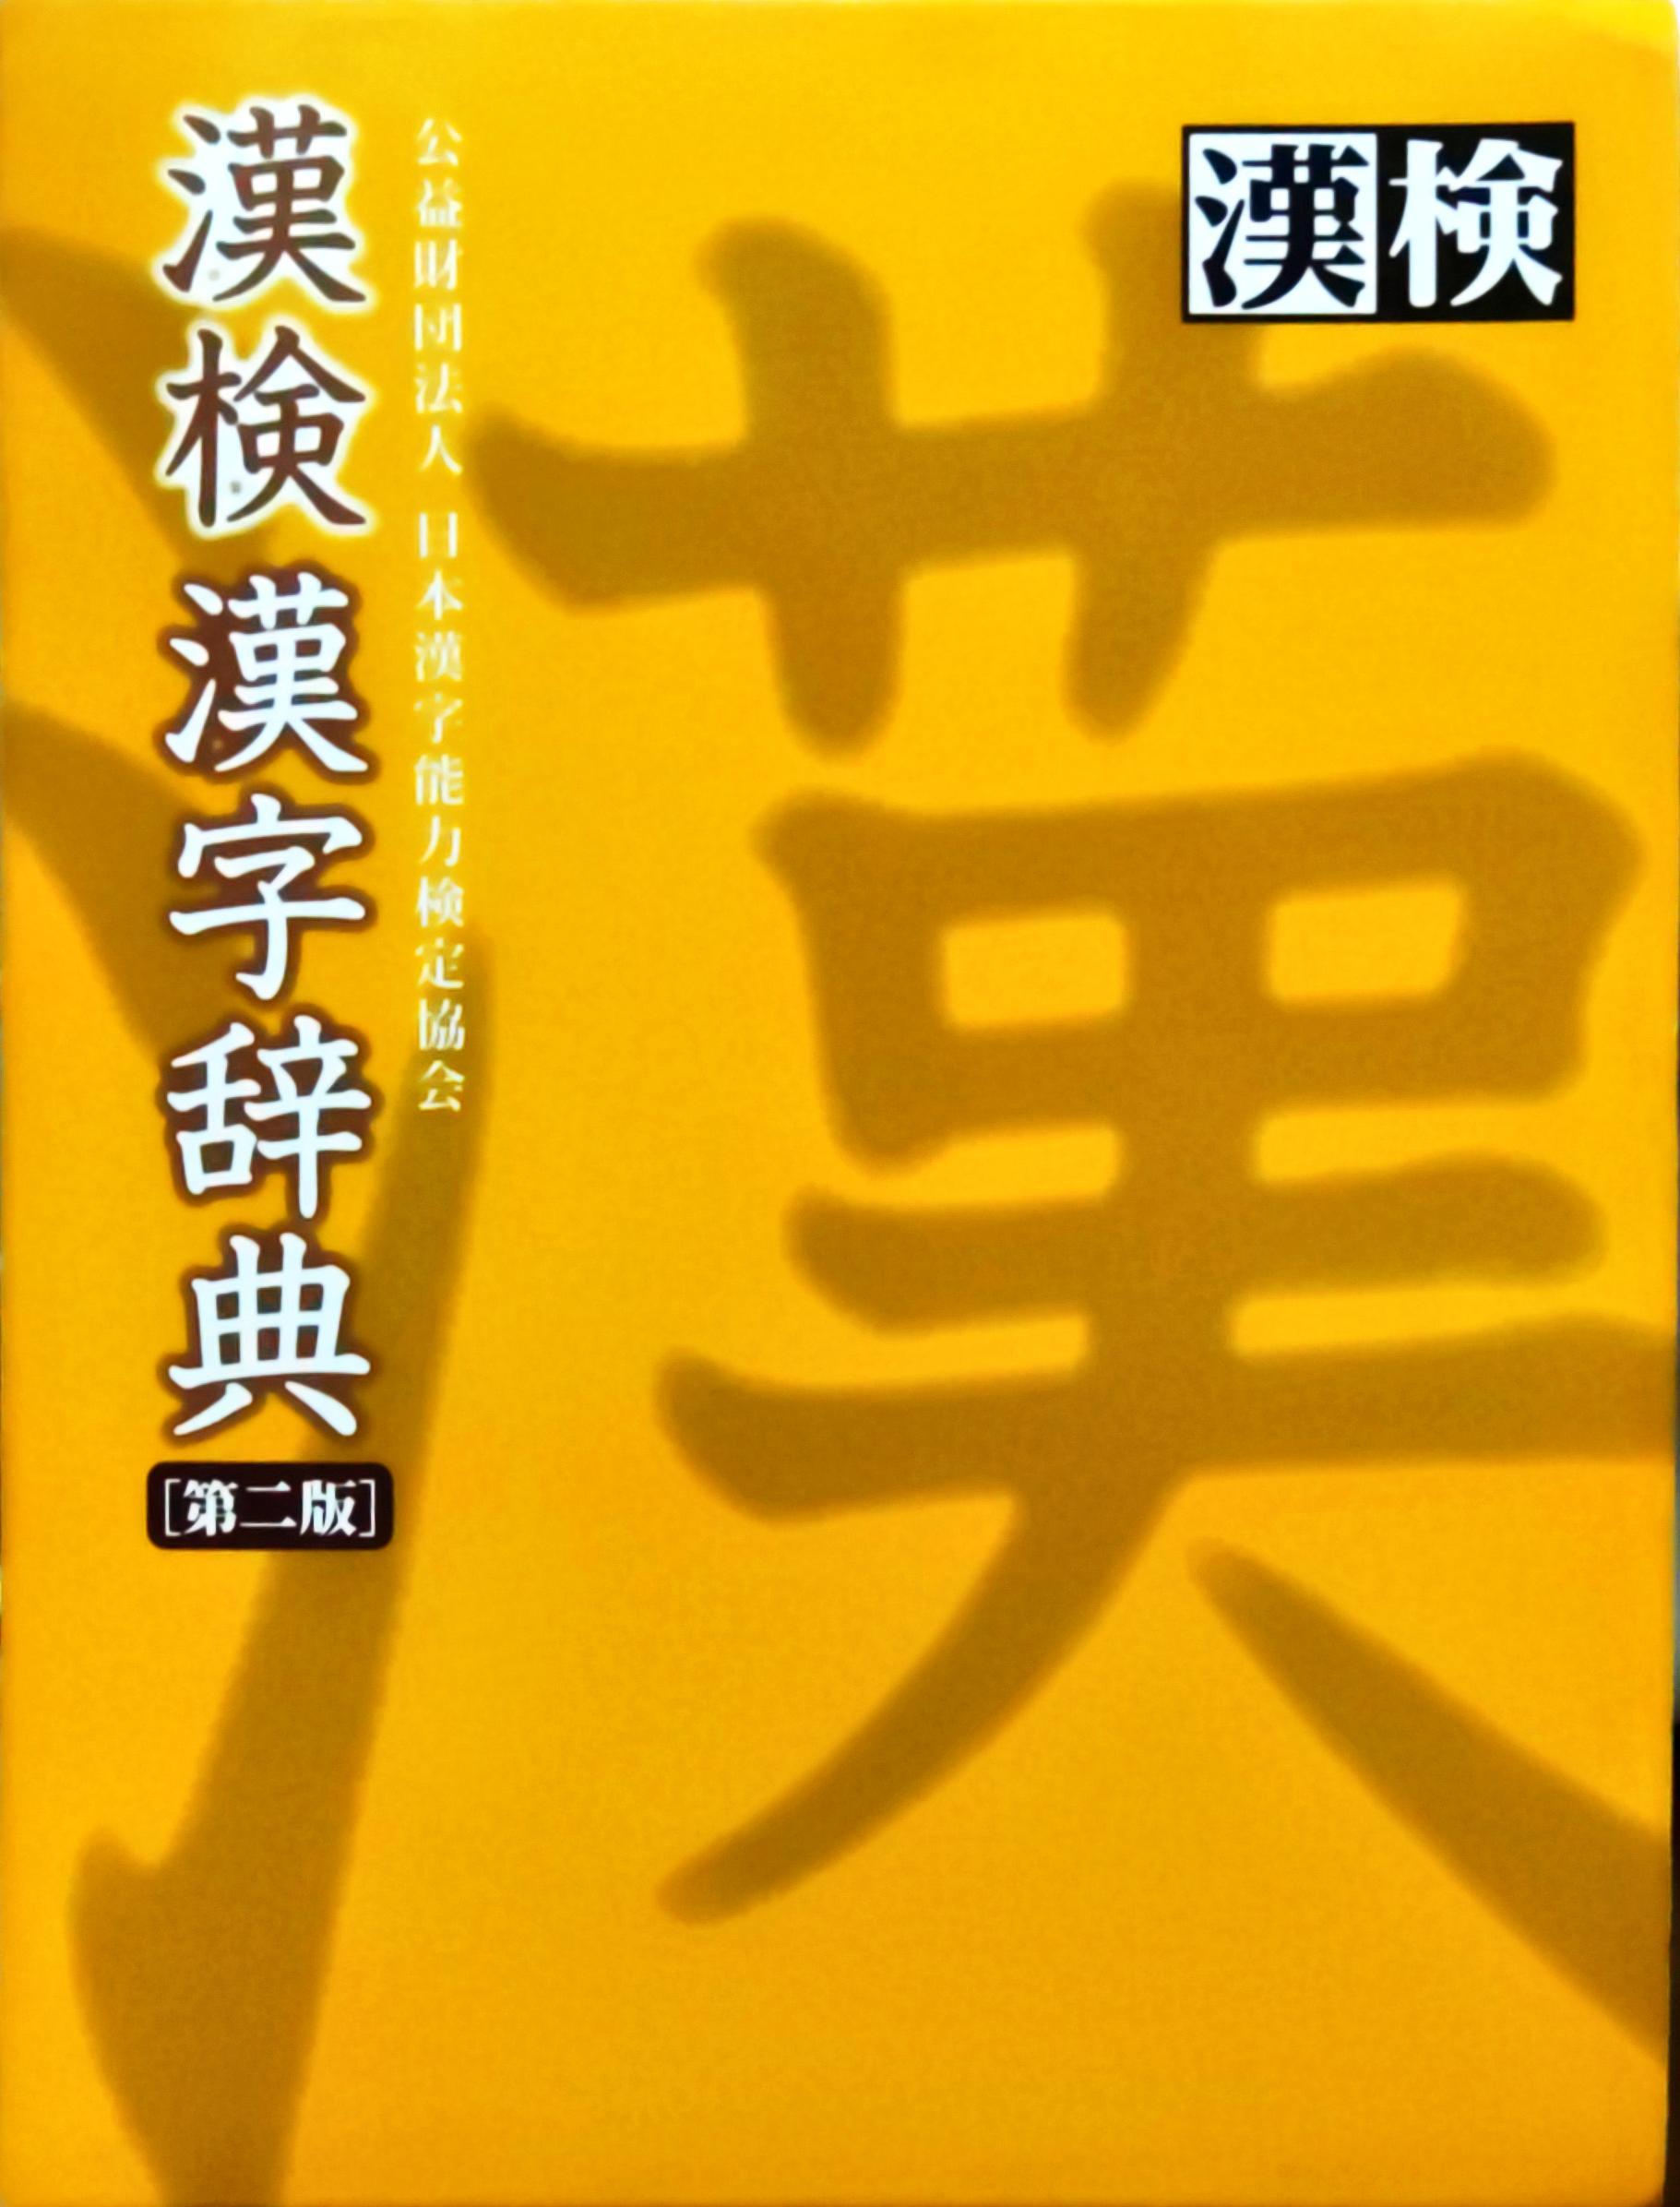
\includegraphics[height=0.8\textheight]{images/kanji-jiten.jpg}
			\end{block}
		\end{column}
			\begin{column}{.6\textwidth}
				\begin{block}{}
					\begin{items}
						\item Kanken Kanji Jiten (Second Edition)
						\item All Kanji will follow this dictionary, and \ruby[m]{常用漢字表}{じょう|よう|かん|じ|ひょう} (Joyo Kanji Table) announced by the Cabinet of Japan.
					\end{items}
				\end{block}
			\end{column}
		\end{columns}
	\end{frame}

	\section{Basics of Kanji}

	\begin{frame}{Basics of Kanji: What is Kanji?}
		\begin{items}
			\item Kanji (\ruby{漢字}{かん|じ}) = Chinese characters
			\item Its origin is unclear.
			\item Japanese started using Kanji around AD 650, and developed \\ \ruby{万葉仮名}{まん|よう|が|な} writing system.
			\item Kanji began its use of sound indication, and certain Kanji evolved into ひらがな and カタカナ.
		\end{items}
	\end{frame}

	\begin{frame}{Origin of Hiragana and Katakana}
		\begin{table}[ht]
			\centering
			\begin{tabular}{cc}
				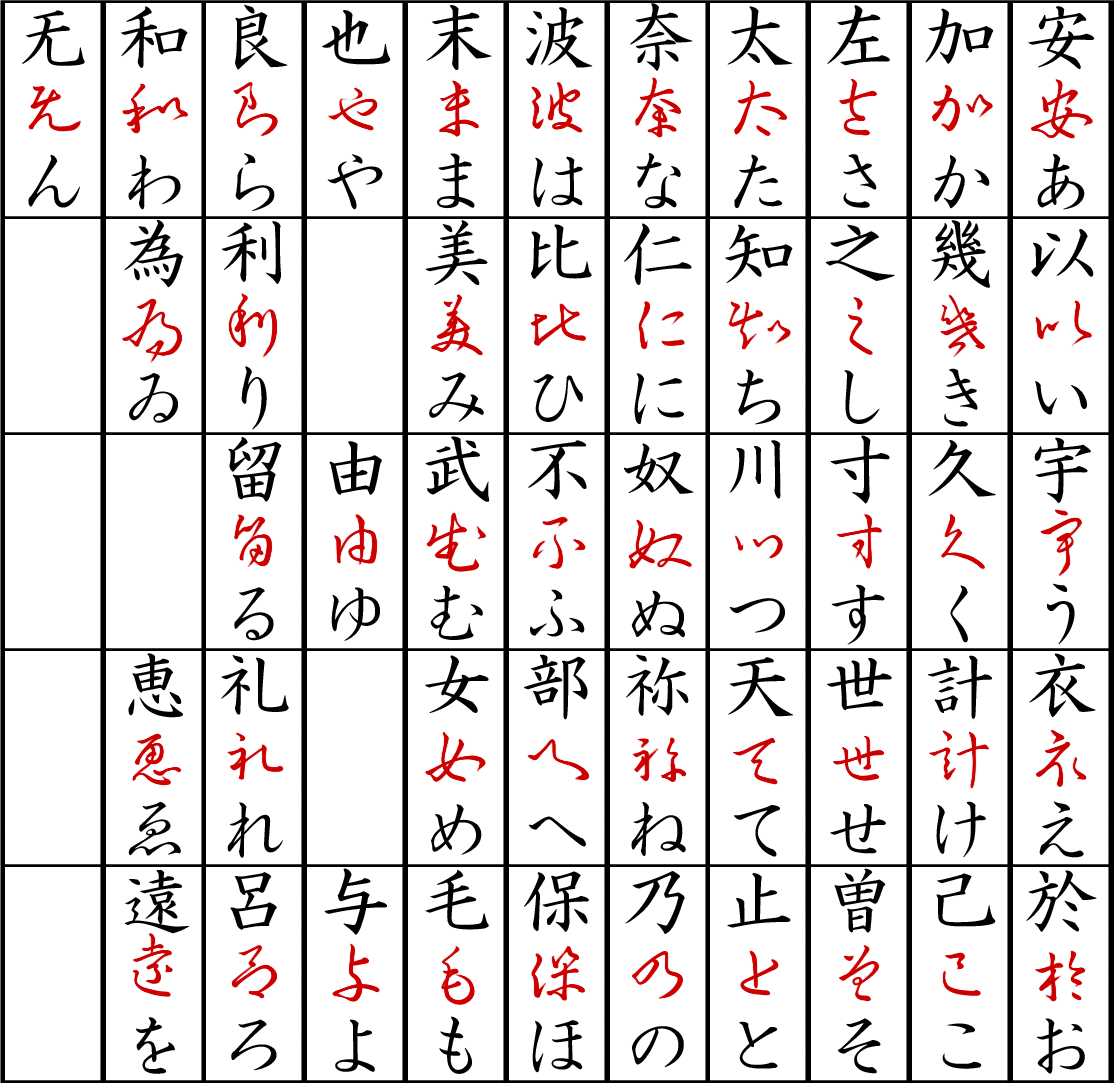
\includegraphics[height=0.75\textheight]{images/Hiragana_origin.png} & 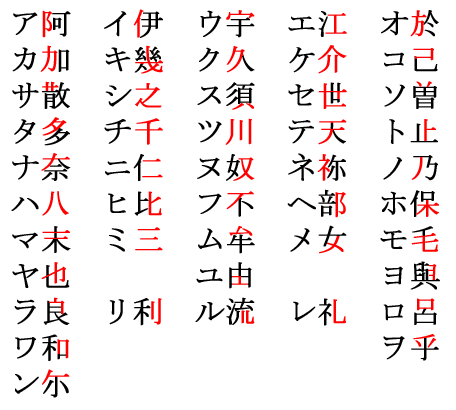
\includegraphics[height=0.75\textheight]{images/Katakana_origin.png}
			\end{tabular}
		\end{table}
	\end{frame}

	\begin{frame}{Basics of Kanji: Classifications of Kanji}
		\begin{items}
			\setlength\itemsep{3pt}
			\item Pictogram (\ruby[m]{象形}{しょう|けい})
			\item Ideogram (\ruby[m]{指事}{し|じ})
			\item Compound (\ruby[m]{会意}{かい|い})
			\item Phono-semantic (\ruby[m]{形声}{けい|せい})
			\item Derivative cognates (\ruby[m]{転注}{てん|ちゅう})
			\item Phonetic loan (\ruby[m]{仮借}{か|しゃ})
		\end{items}
	\end{frame}

	\begin{frame}{Classifications of Kanji: Pictogram}
		\begin{itemize}
			\item Pictogram (\ruby[m]{象形}{しょう|けい}) = Letters representing a picture.
			\item There are about 600 Kanji of this type.
		\end{itemize}
	\end{frame}

	\begin{frame}{Classifications of Kanji: Pictogram}
		\begin{table}[ht]
			\centering
			\begin{tabular}{cc}
				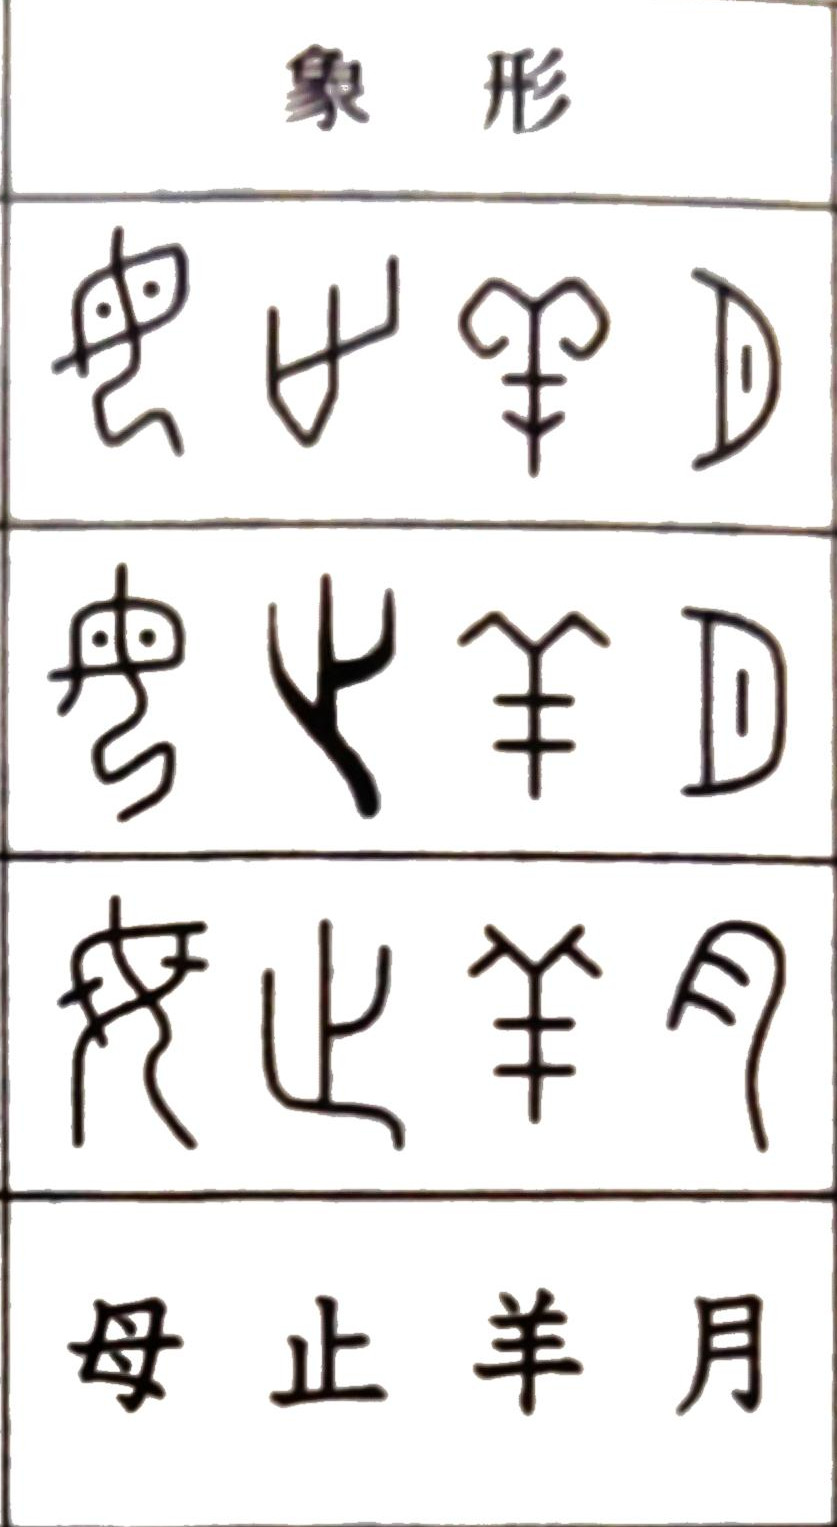
\includegraphics[height=0.8\textheight]{images/shokei-01.jpg} & 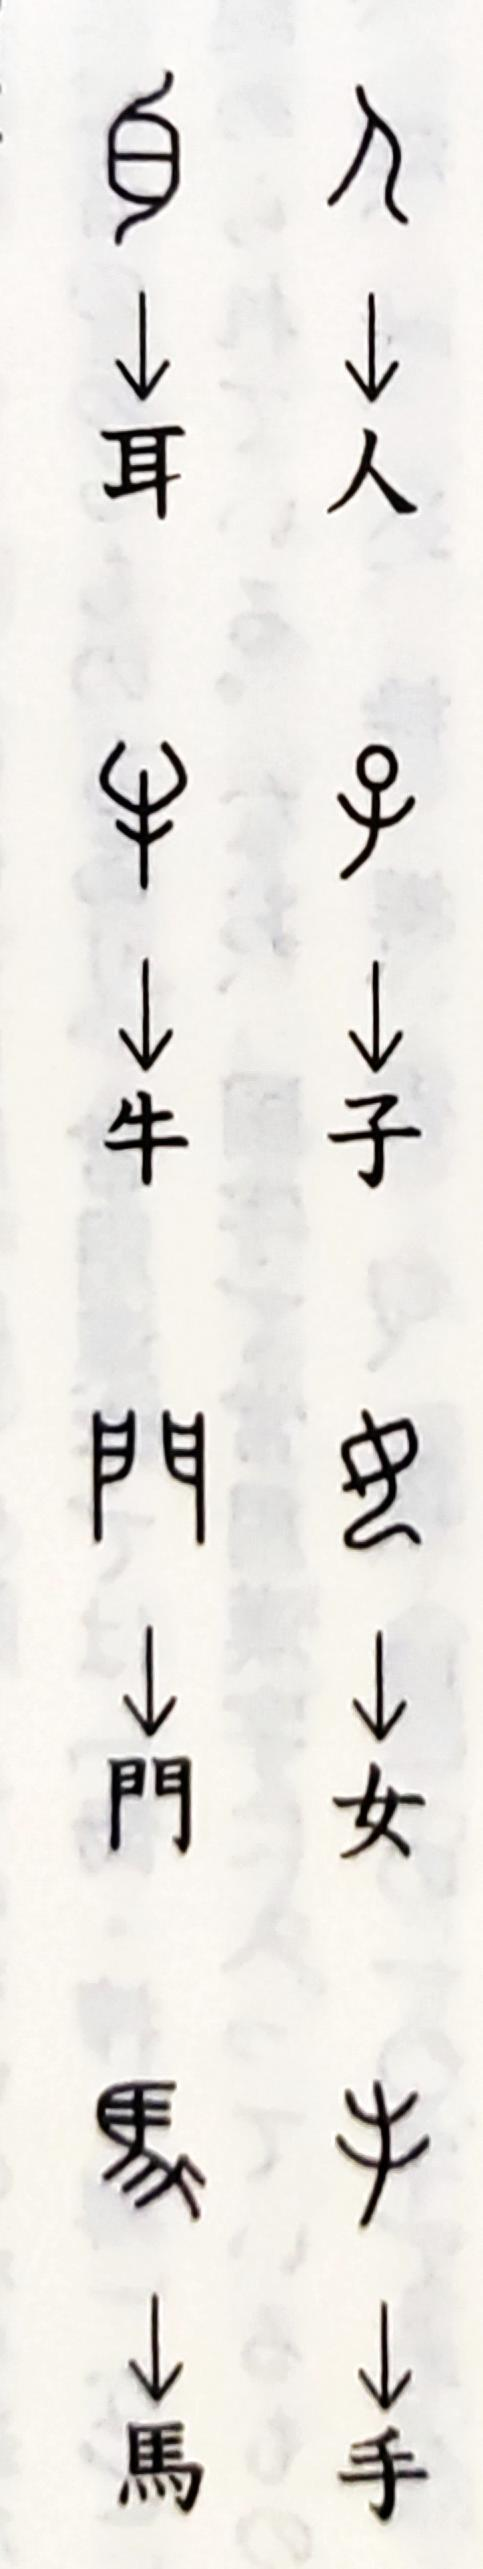
\includegraphics[height=0.8\textheight]{images/shokei-02.jpg}
			\end{tabular}
		\end{table}
	\end{frame}

	\begin{frame}{Classifications of Kanji: Ideogram}
		\begin{itemize}
			\item Ideogram (\ruby[m]{指事}{し|じ}) = Letters which indicate \textbf{abstract ideas}.
			\item Ex. 上 (Up), 下 (Down), 本 (Book, base), 刃 (Blade)
			\item 本 = 木 + 一
			\item 刃 = 刀 + 丶
			\item There are about 120 Kanji of this type.
		\end{itemize}	
	\end{frame}

	\begin{frame}{Classifications of Kanji: Ideogram}
		\begin{table}[ht]
			\centering
			\begin{tabular}{cc}
				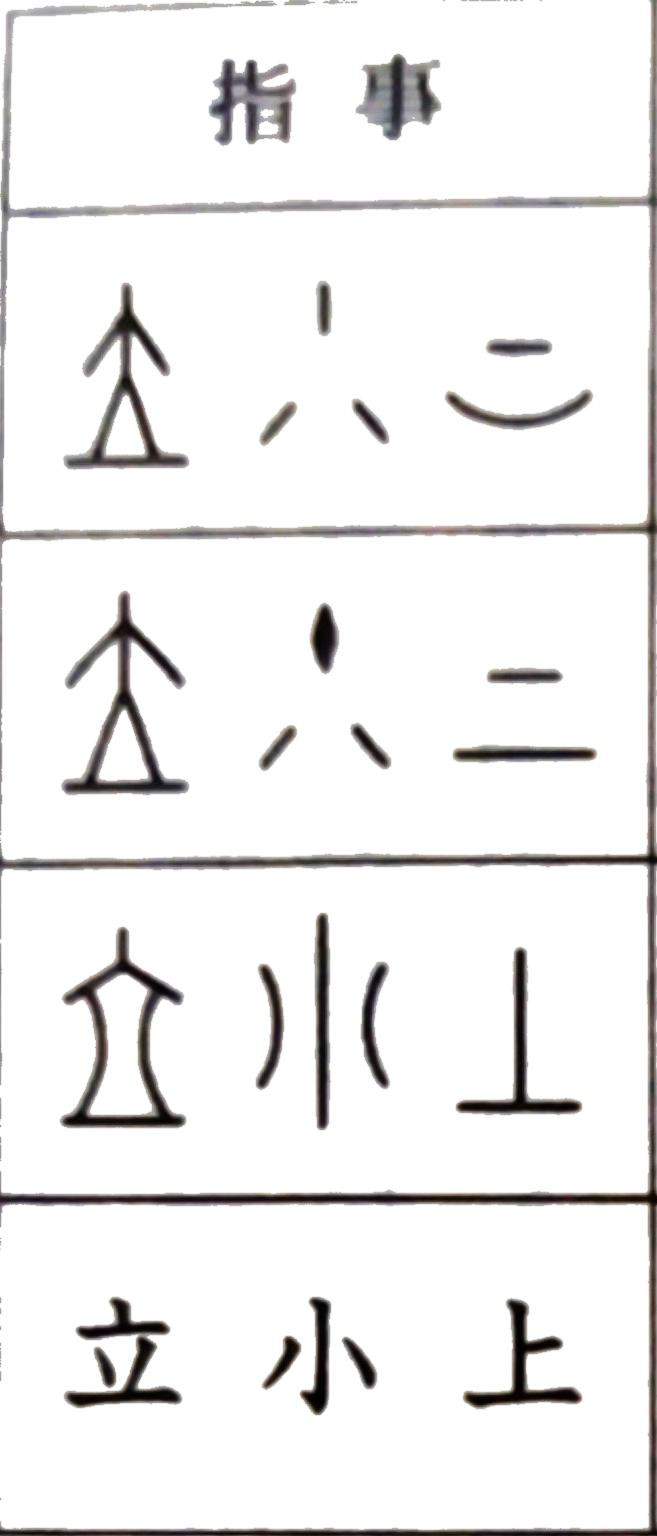
\includegraphics[height=0.8\textheight]{images/shiji-01.jpg} & 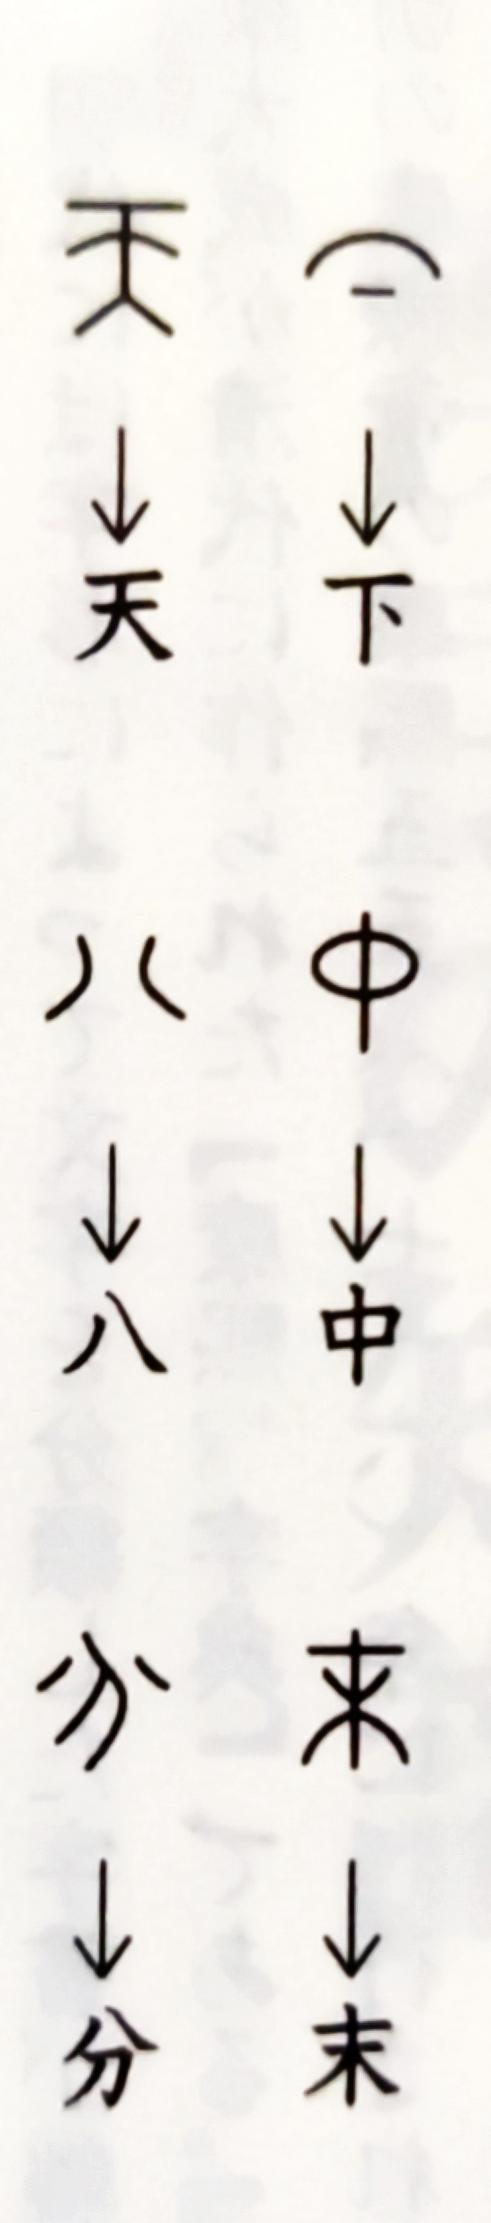
\includegraphics[height=0.8\textheight]{images/shiji-02.jpg}
			\end{tabular}
		\end{table}
	\end{frame}

	\begin{frame}{Classifications of Kanji: Compound}
		\begin{itemize}
			\item Compound (\ruby[m]{会意}{かい|い}) = Kanji made up of 2 or more Pictogram and Ideogram.
			\item Newly made Kanji will have new meanings and pronunciation.
			\item 日 (Sun) + 月 (Moon) = 明 (Bright)
			\item 木 (Tree) + 木 (Tree) = 林 (Wood)
			\item 木 (Tree) + 木 (Tree) + 木 (Tree) = 森 (Forest)
		\end{itemize}	
	\end{frame}

	\begin{frame}{Classifications of Kanji: Compound}
		\begin{itemize}
			\item Some Compound Kanji are Made in Japan.
			\item Japanese-made Kanji = \ruby[m]{国字}{こく|じ}
			\item 働 (Labor) = 亻 (Person) + 動 (Move)
			\item 畑 (Field) = 火 (Fire) + 田 (Rice field)
			\item 峠 (Mountain pass) = 山 (Mountain) + 上 (Up) + 下 (Down)
		\end{itemize}	
	\end{frame}

	\begin{frame}{Classifications of Kanji: Ideogram}
	\begin{table}[ht]
		\centering
		\begin{tabular}{cc}
			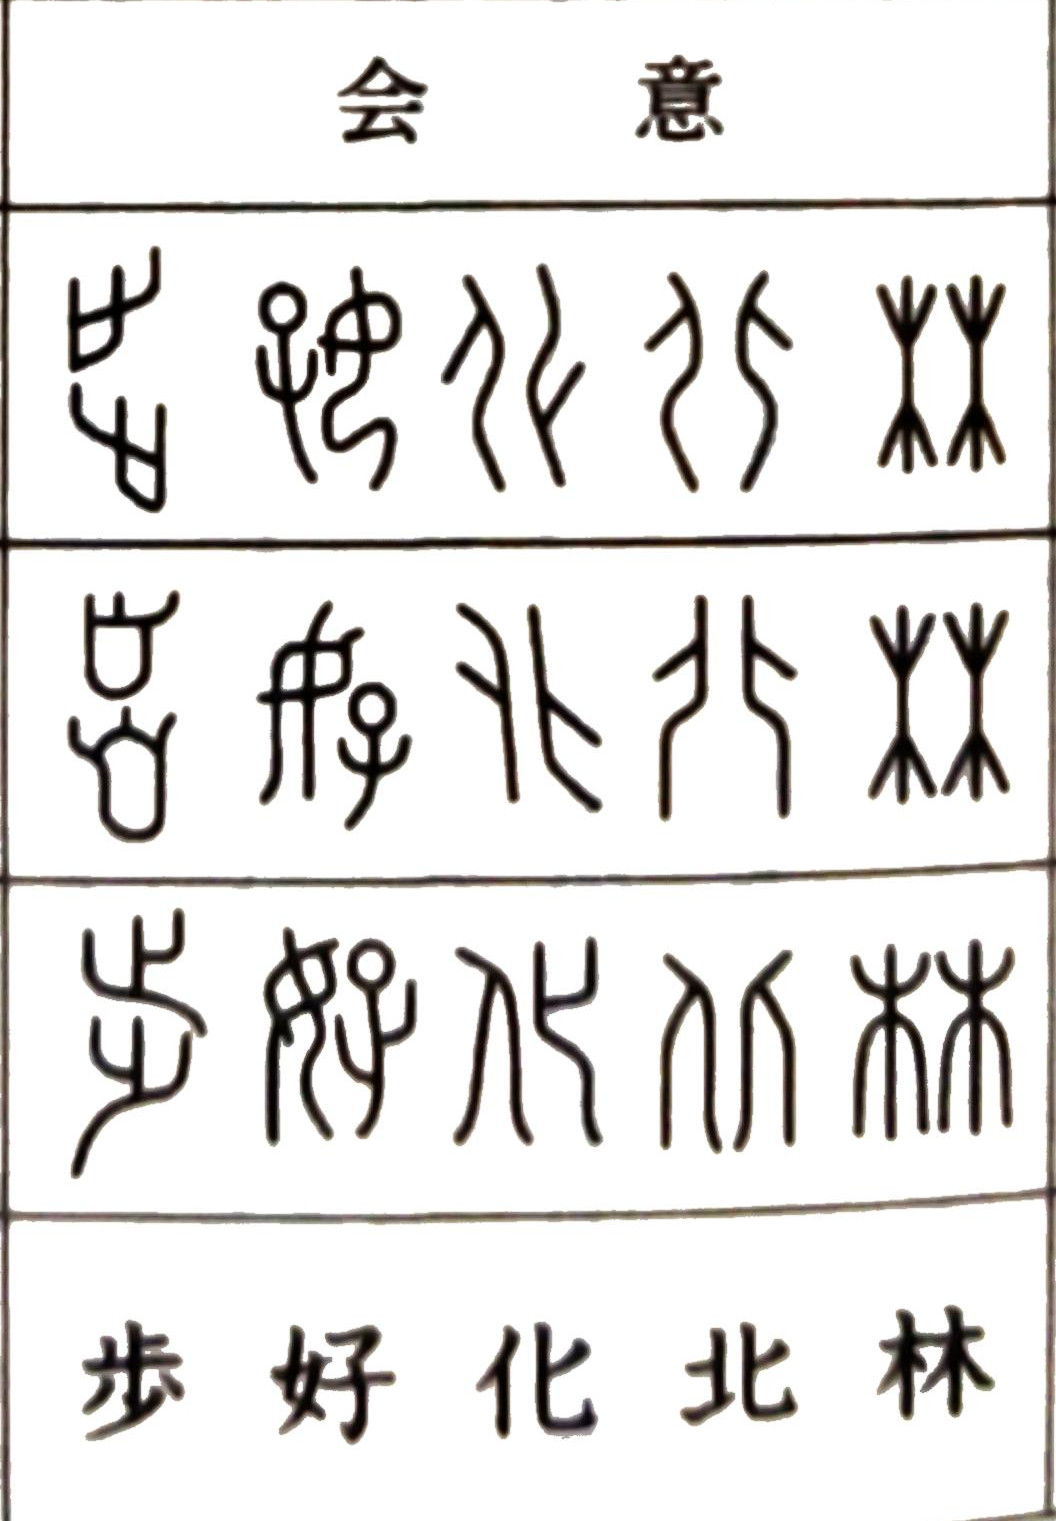
\includegraphics[height=0.8\textheight]{images/kaii-01.jpg} & 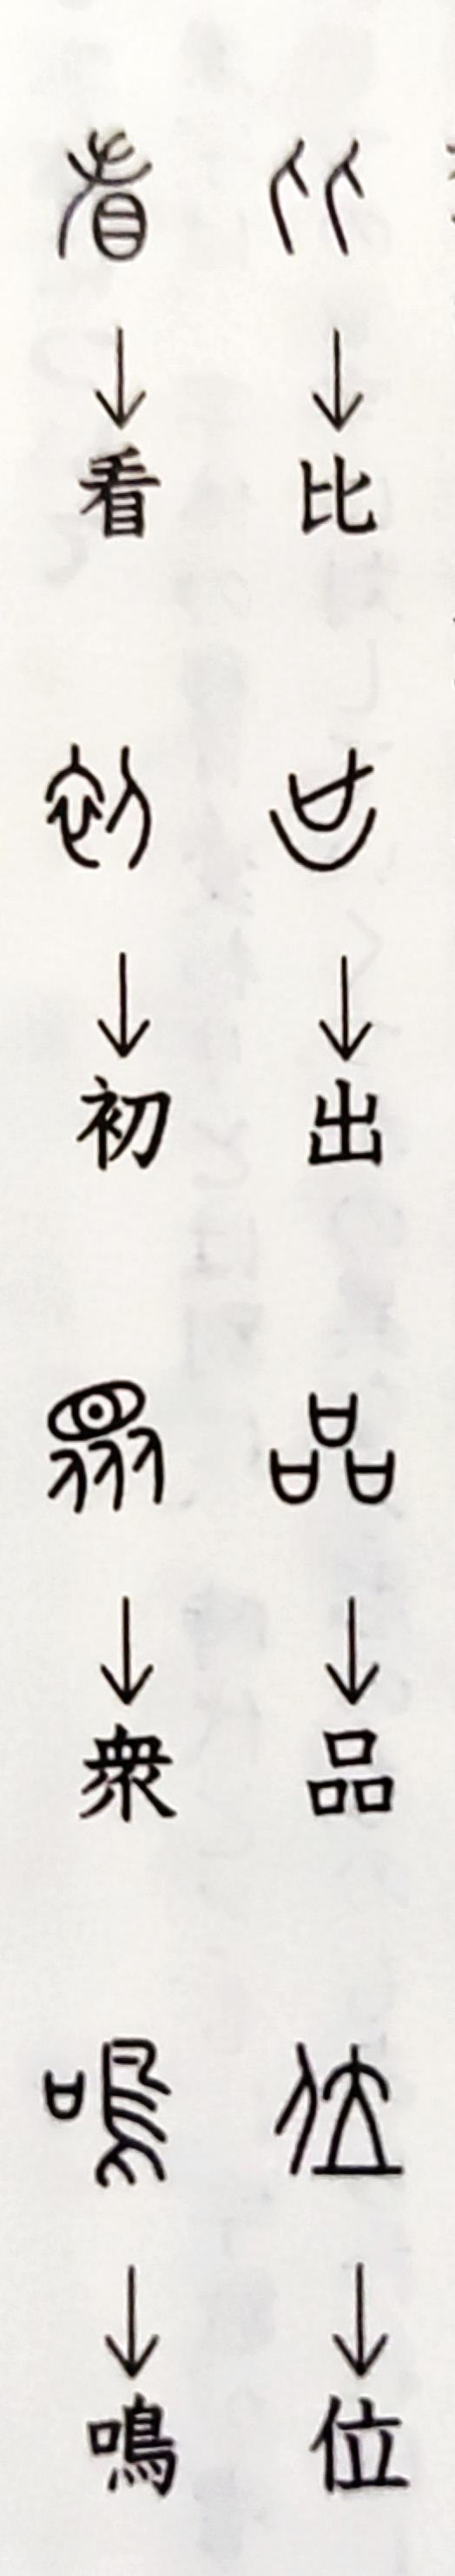
\includegraphics[height=0.8\textheight]{images/kaii-02.jpg}
		\end{tabular}
	\end{table}
	\end{frame}

	\begin{frame}{Classifications of Kanji: Phono-semantic}
		\begin{itemize}
			\item Phono-semantic (\ruby[m]{形声}{けい|せい}) = Kanji made from 2 parts.
			\begin{itemize}
				\item Meaning part.
				\item Sound part.
			\end{itemize}
			\item About 80\% of Kanji belong to this category.
		\end{itemize}	
	\end{frame}

	\begin{frame}{Classifications of Kanji: Phono-semantic}
	\begin{table}[ht]
		\centering
		\begin{tabular}{|c|c|c|c|}
			\hline
			\textbf{Meaning part} & \textbf{Sound part} & \textbf{Kanji} & \textbf{Meaning} \\
			\hline
			\multirow{2}{*}{氵 (Water)} & 可 (カ) & 河 & River \\
			 & 先 (セン) & 洗 & Wash \\
			\hline
			\multirow{2}{*}{木 (Tree)} & 反 (ハン) & 板 & Board \\
			& 主 (チュウ) & 柱 & Pillar \\
			\hline
			\multirow{2}{*}{糸 (Thread, yarn)} & 吉 (ケツ) & 結 & Tie, unite \\
			& 扁 (ヘン) & 編 & Knit \\
			\hline
		\end{tabular}
	\end{table}
	\end{frame}

	\begin{frame}{Classifications of Kanji: Phono-semantic}
		\begin{itemize}
			\item Some Phono-semantic Kanji consist of a sound part which has its own meaning. As a subcategory, this kind of Kanji is called "Compound Phono-semantic" (\ruby[m]{会意形声}{かい|い|けい|せい})
			\item 圣 (ケイ) means "straight"
			\item 青 (セイ) means "blue, clear"
		\end{itemize}
	\end{frame}

	\begin{frame}{Classifications of Kanji: Phono-semantic}
	\begin{table}[ht]
		\centering
		\begin{tabular}{|c|c|c|c|}
			\hline
			\textbf{Part 1} & \textbf{Part 2} & \textbf{Kanji} & \textbf{Meaning} \\
			\hline
			\multirow{3}{*}{圣 (ケイ)} & 艹 & 茎 & Stalk \\
			& 彳 & 径 & Straight, small path \\
			& 車 & 軽 & Going straight, light car \\
			\hline
			\multirow{3}{*}{青 (セイ)} & 氵 & 清 & Clear water \\
			& 日 & 晴 & Clear sky \\
			& 争 & 静 & Peaceful (clear of quarrel) \\
			\hline
		\end{tabular}
	\end{table}
	\end{frame}

	\begin{frame}{Types of Phono-semantic}
		\begin{itemize}
			\item Phono-semantic Kanji consist of 2 parts:
			\begin{itemize}
				\item Meaning part
				\item Sound part
			\end{itemize}
			\item These two parts have 8 ways of combination depending on their positions.
		\end{itemize}
	\end{frame}

	\begin{frame}{Combinations of Phono-semantic Kanji}
		\begin{table}[ht]
			\centering
			\begin{tabular}{|c|c|c|c|c|}
				\hline
				\textbf{No.} & \textbf{Meaning part} & \textbf{Sound part} & \textbf{Examples} & \textbf{Combination} \\
				\hline
				1 & Left side & Right side & 鋼 (コウ) & 金 + 岡 \\
				 & & & 体 (タイ) & 亻 + 本 \\
				 & & & 悟 (ゴ) & 忄 + 吾 \\
				\hline
				2 & Right side & Left side & 敗 (ハイ) & 貝 + 攵 \\
				 & & & 彩 (サイ) & 采 + 彡 \\
				 & & & 戦 (セン) & 単 + 戈 \\
				\hline
			\end{tabular}
		\end{table}
	\end{frame}

	\begin{frame}{Combinations of Phono-semantic Kanji}
	\begin{table}[ht]
		\centering
		\begin{tabular}{|c|c|c|c|c|}
			\hline
			\textbf{No.} & \textbf{Meaning part} & \textbf{Sound part} & \textbf{Examples} & \textbf{Combination} \\
			\hline
			3 & Above & Bottom & 管 (カン) & 竹 + 官 \\
			& & & 崩 (ホウ) & 山 + 朋 \\
			& & & 突 (トツ) & 穴 + 大  \\
			\hline
			4 & Bottom & Above & 型 (ケイ) & 土 + 刑 \\
			& & & 想 (ソウ) & 	心 + 相  \\
			& & & 響 (キョウ) & 音 + 郷 \\
			\hline
		\end{tabular}
	\end{table}
	\end{frame}

	\begin{frame}{Combinations of Phono-semantic Kanji}
	\begin{table}[ht]
		\centering
		\begin{tabular}{|c|c|c|c|c|}
			\hline
			\textbf{No.} & \textbf{Meaning part} & \textbf{Sound part} & \textbf{Examples} & \textbf{Combination} \\
			\hline
			5 & Outside & Inside & 圏 (ケン) & 囗 + 巻 \\
			& & & 街 (ガイ) & 行 + 圭 \\
			& & & 匿 (トク) & 匚 + 若  \\
			\hline
			6 & Inside & Outside & 聞 (モン) & 耳 + 門 \\
			& & & 気 (キ) & メ + 气  \\
			\hline
		\end{tabular}
	\end{table}
	\end{frame}

	\begin{frame}{Combinations of Phono-semantic Kanji}
	\begin{table}[ht]
		\centering
		\begin{tabular}{|c|c|c|c|c|}
			\hline
			\textbf{No.} & \textbf{Meaning part} & \textbf{Sound part} & \textbf{Examples} & \textbf{Combination} \\
			\hline
			7 & - & Top-right & 趣 (シュ) & 走 + 取 \\
			& & & 近 (キン) & 辶 + 斤 \\
			& & & 魅 (ミ) & 鬼 + 未  \\
			\hline
			8 & - & Bottom-right & 房 (ボウ) & 戸 + 方 \\
			& & & 庭 (テイ) & 广 + 廷  \\
			& & & 癖 (ヘキ) & 疒 + 辟  \\
			\hline
		\end{tabular}
	\end{table}
	\end{frame}

	\begin{frame}{Classifications of Kanji: Derivative Cognates}
		\begin{itemize}
			\item Derivative cognates (\ruby[m]{転注}{てん|ちゅう}) = Extending the original meaning of Kanji into a new one, regardless of the origin of that character.
		\end{itemize}
	\end{frame}

	\begin{frame}{Examples of Derivative Cognates}
		\begin{table}[ht]
			\centering
			\begin{tabular}{|c|c|c|}
				\hline
				\textbf{Kanji} & \textbf{Original meaning} & \textbf{New meaning} \\
				\hline
				楽 & Music (\ruby[m]{音楽}{おん|がく}) & Fun (\ruby{楽}{たの}しい) \\
				\hline
				悪 & Bad (\ruby{悪}{わる}い) & Hate (\ruby[m]{嫌悪}{けん|お}) \\
				\hline
				好 & Good (\ruby{好}{よ}い) & Like (\ruby{好}{この}む) \\
				\hline
				節 & Section (of bamboo) (\ruby{節}{ふし}) & Chastity (\ruby[m]{貞節}{てい|せつ}) \\
				\hline
			\end{tabular}
		\end{table}
	\end{frame}

	\begin{frame}{Classifications of Kanji: Phonetic Loan}
		\begin{itemize}
			\item Phonetic loan (\ruby[m]{仮借}{か|しゃ}) = Using a Kanji in a completely different meaning by borrowing its sound.
			\item This also includes foreign words like country names, which are similar to how Chinese use Hanzi to represent the sound of these words.
			\item \ruby[m]{印度}{イン|ド} = India
			\item \ruby[g]{英吉利}{イギリス} = United Kingdom -> \ruby{英}{エイ}
			\item \ruby[g]{亜米利加}{アメリカ} = USA -> \ruby{米}{ベイ}
		\end{itemize}
	\end{frame}
	
	\begin{frame}{Examples of Phonetic Loan}
		\begin{table}[ht]
			\centering
			\begin{tabular}{|c|c|c|c|}
				\hline
				\textbf{Kanji} & \textbf{Sound} & \textbf{Original meaning} & \textbf{New meaning} \\
				\hline
				東 & トウ & Bag tied with a stick & East \\
				\hline
				豆 & トウ & A tableware & Bean \\
				\hline
				来 (來) & ライ & Wheat & Come \\
				\hline
			\end{tabular}
		\end{table}
	\end{frame}

	\begin{frame}{Next Class}
		\begin{itemize}
			\item Radical (\ruby[m]{部首}{ぶ|しゅ})
			\item Sounds of Kanji (\ruby[m]{音読}{おん|よ}み、\ruby[m]{訓読}{くん|よ}み)
			\item Kanji compound (\ruby[m]{熟語}{じゅく|ご})
		\end{itemize}
	\end{frame}

\end{document}
